% Pre-results research draft. Compile with an IEEEtran conference class.
% This file intentionally contains explicit result placeholders.
\documentclass[conference,a4paper,10pt]{IEEEtran}
\usepackage{amsmath,amssymb,graphicx,booktabs,array,url}
\newcommand{\pending}{\textsc{Not yet measured}}
\newcommand{\insuff}{\textsc{Insufficient validated evidence}}
\newcommand{\placeholder}[2]{\fbox{\begin{minipage}{0.91\columnwidth}\centering\textbf{#1}\\[3pt]\footnotesize #2\end{minipage}}}
\title{SecureLLMBench: A Traceable and Validation-Aware Platform for Reproducible LLM Security Evaluation}
\author{\IEEEauthorblockN{[AUTHOR NAME]}\IEEEauthorblockA{[DEPARTMENT]\\[INSTITUTION]\\[LOCATION]\\[EMAIL]}}
\begin{document}
\maketitle
\begin{abstract}
Deployed language-model assistants may encounter adversarial user conversations while operating under confidential application instructions. An immediate jailbreak-success score does not necessarily measure whether an earlier adversarial exchange affects a later, legitimate request. This paper presents SecureLLMBench as an implemented, provenance-aware research backend and specifies a controlled feasibility study of downstream synthetic-secret disclosure. The proposed study compares live adversarial histories with topic-matched benign histories, generic benign histories, benign-refusal histories, and isolated-attack controls; scripted-history replay remains a separate mechanism study. At a final legitimate probe, an objective-specific checker would distinguish exact disclosure from earlier leakage, invalid responses, and broader semantic disclosures. The initial specification targets local Qwen3.5:2b and Gemma3:4b models at zero, two, and five benign filler exchanges, with paired goal-level analysis and explicit context-integrity gates. The existing backend stores ordered observations and supports immutable evidence and null-preserving metric reporting, but the new checker, intervention arms, and model-specific prompt-rendering verification have not been implemented. A historical judge comparison is independently reproducible and shows limited agreement under its fixed mapping; it does not answer the proposed research question. \textbf{[RESULTS PENDING --- INSERT VERIFIED PILOT OR CONFIRMATORY FINDINGS]} The intended contribution is a controlled and auditable measurement design whose empirical claims remain conditional on completed execution and validated evidence.
\end{abstract}
\begin{IEEEkeywords}
large language models, LLM security, prompt injection, jailbreak evaluation, adversarial conversation history, security benchmarking, contextual influence, reproducibility
\end{IEEEkeywords}

\section{Introduction}
Language-model assistants can maintain conversation state while following application instructions that users should not override. A harmful request can be refused immediately yet still alter what text remains in a later context; conversely, a later violation could simply reflect a difficult benign task or a secret already leaked earlier. A single response-level success rate does not distinguish these possibilities. Standardized jailbreak benchmarks establish useful attack datasets and scoring protocols \cite{jbb,harmbench}, but an evaluation of delayed disclosure needs its own outcome and an explicit counterfactual history.

We consider an attacker who supplies user messages before a legitimate final task while a defender has been instructed to keep a synthetic secret confidential. The primary comparison is between a live adversarial history and a topic-matched benign history, with the same model, goal, final task, and post-exposure distance. The topic-matched arm matters because a generic benign conversation may differ in subject matter, vocabulary, and available cues. We additionally plan refusal-history and isolated-attack arms to diagnose alternative explanations; these are not substitutes for the primary comparator. Earlier defender responses remain part of the trajectory even if they already expose the secret.

The specific question is whether adversarial history changes the probability of exact disclosure in the designated final response, and whether this excess risk changes after benign filler exchanges. We call the latter comparison \emph{contextual influence decay}. It is a property of responses under constructed prompts, not evidence that model weights or persistent memory changed. Prompt-template behavior and context retention can confound an apparent distance effect; the design therefore requires model-specific rendering evidence and explicit truncation status. Work on long-context positional effects makes that concern concrete \cite{lostmiddle}.

SecureLLMBench already includes local inference adapters, a controlled trajectory runner, immutable observations, dataset/protocol hashes, metric applicability rules, and evidence-gated reports. The present manuscript separates those implemented software properties from a \emph{proposed} delayed-disclosure study. It contributes an inspectable estimand and a set of falsifiable gates for future observations. It does not report that the study has run, establish an attack effect, or recommend a safer model.

\section{Related Work}
\subsection{Jailbreak benchmarking and evaluation}
JailbreakBench provides a standardized threat model, attack artifacts, behaviors, scoring functions, and templates \cite{jbb}. HarmBench studies automated red teaming and robust refusal at substantially larger scale \cite{harmbench}. These systems make clear that benchmark comparability depends on the complete evaluation configuration, not a model name alone. Their existence precludes any claim that open jailbreak benchmarking itself is new here. The proposed outcome instead isolates a delayed exact disclosure under a fixed trusted instruction and an otherwise legitimate final probe.

\subsection{Multi-turn adversarial evaluation}
Multi-turn safety and recovery questions are already active research topics; a delayed effect is not novel by terminology alone. A multi-turn attack can change both the text seen at the final probe and the model's own intervening replies. Consequently, a single final prompt does not identify which earlier exchange supplied an apparent effect. Our live arm retains all defender replies and records an outcome after exposure ends. A scripted assistant history is useful as a separate mechanism probe, but it is not a live defender continuation and will not be pooled with it. A review of additional specialized multi-turn benchmarks remains necessary before claiming a distinct research niche.

\subsection{Prompt injection and downstream failures}
AgentDojo evaluates attacks against tool-using agents in dynamic tasks \cite{agentdojo}, while InjecAgent studies indirect injections in tool-integrated agents \cite{injecagent}. Those threat models involve attacker-controlled external or tool material rather than the user-only attacker specified here. They nevertheless show why security outcomes should be tied to explicit application objectives. Tool execution and exact secret emission have different opportunities for observation and different false-positive modes. The proposed study therefore compares its own matched conditions, not cross-paper success percentages.

\subsection{Context position and retention}
Lost in the Middle demonstrates that the position of relevant information can affect long-context performance \cite{lostmiddle}. The proposed distances therefore need token-distance controls and context evidence before a trend can be interpreted. A turn-count difference is not necessarily a token-distance difference: model-specific templates, generated refusal length and filler response length can alter the effective prompt. Even complete client-side message logs do not certify retained model context. These variables require explicit recording and sensitivity analysis rather than an assumption that a declared context window is fully available.

\subsection{Automated evaluator reliability}
StrongREJECT documents ways automated jailbreak evaluators can overstate success and validates an evaluator against human judgments \cite{strongreject}. In our repository, a separate historical Gemma-based safety-stance comparison has only modest agreement with its reference labels (Sec.~\ref{sec:existing-evidence}); it is not a validated substitute for independent semantic labels in this new task. Exact synthetic-secret matching avoids an LLM judge for the narrow primary event, though it cannot capture all information leakage. The exact checker itself requires adversarial positive, negative and near-miss fixture validation before use.

\subsection{Research gap and positioning}
The open empirical question is not whether language models can be attacked, or whether long contexts influence outputs. It is whether a live adversarial history produces excess \emph{later} exact disclosure relative to a history matched for the same legitimate task, subject matter and distance. Existing systems motivate the question but do not supply observations for this particular estimand. The manuscript treats that estimand as a proposed test, not as an established novelty result. A pre-submission review must check whether an equivalent contrast has already been published and update the positioning accordingly.

\begin{table*}[!t]
\caption{Related-work feature comparison. ``Not verified'' means the cited source was not confirmed to establish the feature; it is not an absence claim. The final row is a proposed protocol, not an executed result.}
\label{tab:related}
\centering\footnotesize
\begin{tabular}{p{2.4cm}p{1.25cm}p{1.25cm}p{1.5cm}p{1.8cm}p{1.4cm}p{3.3cm}}
\toprule
Study & Multi-turn & Live replies & Delayed probes & Matched benign controls & Objective checker & Main outcome \\
\midrule
JailbreakBench \cite{jbb} & Not verified & Not verified & Not verified & Not verified & Scoring functions & Jailbreak behavior success \\
HarmBench \cite{harmbench} & Not verified & Not verified & Not verified & Not verified & Automated evaluation & Red-teaming/refusal evaluation \\
AgentDojo \cite{agentdojo} & Dynamic agent tasks & Yes, agent execution & Not verified & Benign tasks exist; matching not verified & Task/security checks & Agent-task and security outcomes \\
InjecAgent \cite{injecagent} & Tool-agent interaction & Yes, agent execution & Not verified & Not verified & Attack-intent checks & Indirect-injection outcomes \\
SecureLLMBench proposal & Yes & Planned & Planned, $d=0,2,5$ & Planned T and R & Planned exact-secret checker & Final/earlier/ever disclosure \\
\bottomrule
\end{tabular}
\end{table*}

The table is deliberately conservative: a feature not verified from a source is not labeled absent. A broader pre-submission literature comparison must test whether existing work already combines equivalent delayed probes, matched histories, and objective-specific checking. The implementation of controls is an engineering capability; their scientific value requires observed contrasts and uncertainty.

There are two distinct comparison dimensions in this literature. First, a benchmark may preserve an attack string, target model and immediate response well enough to reproduce an attack-success decision. Second, an application-oriented study may need a legitimate future task, a maintained trusted instruction and a non-adversarial history with the same task context. Evidence for the first does not imply evidence for the second. The related-work table therefore avoids interpreting an unspecified delayed probe as absent, and avoids treating an agent tool action as directly comparable to a conversational exact-string event. The planned contribution is a measured contrast, if one emerges, rather than a claim of priority over these systems.

Evaluator reliability also changes which comparisons are scientifically possible. A refusal detector, safety-stance judge and objective-success judge label different constructs. StrongREJECT's concern with vacuous harmful-looking answers \cite{strongreject} is a warning against treating non-refusal as fulfilled attacker intent. The planned exact-secret event has a crisp string-level target and can be checked without a new judge, but the broader question of whether a response conveys confidential information remains open. This distinction motivates reporting exact, canonicalized and semantic categories separately rather than collapsing them into one success score after observing outputs.

\section{SecureLLMBench Architecture}
The ordinary benchmark route reads a processed dataset, resolves a model from the registry, calls an inference provider, and stores individual responses, latency, and execution status. \texttt{core/benchmark/engine.py} does not itself compute a validated security outcome. Its three-case local demonstration is useful for execution checks, not a population estimate. The research route is different: \texttt{core/experiments/runner.py} builds controlled baseline, isolated, sequential, recovery, and benign-control lanes, sends ordered conversations, and saves immutable observation records. \texttt{scripts/run\_controlled\_experiment.py} checks a source hash, local protocol lock, installed model identity, and call cap before execution. These existing lanes do not yet implement the proposed seven-arm secret-disclosure study.

The Ollama adapter sends message roles and generation options through \texttt{/api/chat}; it records provider token counts and a request-level context status. A count below the declared context window does not prove which tokens survived template rendering or were used by the model. The adapter currently lacks top-p in its shared generation contract. The manifest records model/configuration identities, seeds, software and artifact hashes. The observation store rejects duplicate IDs, while scientific records are appended under typed families. These features make results traceable but do not make an outcome scientifically valid by themselves.

The repository also separates source identity from execution identity. A source dataset can be SHA-256 checked before a run, while each observation carries experiment, run, case, model, condition, generation and time fields. Resuming the controlled runner reuses completed observation IDs and refuses to overwrite an existing record. This reduces accidental replacement of inconvenient observations, although filesystem permissions and external copies remain operational responsibilities. A manifest can describe requested and effective seeds, software versions, observation hashes and unavailable metadata. An analyst must still verify that a record belongs to the intended evidence class before it enters a paper table.

The backend's scientific-record table is append-oriented and keeps measurement families apart. It is therefore possible to preserve a failed response, an undefined behavioral state and a completed provider call as distinct facts. The reporting layer uses provenance classes to exclude fixtures and engineering pilots from paper-ready plots. That is an eligibility rule, not a statistical correction. In particular, the proposed final exact-disclosure outcome would need its own schema, versioned checker, trial-secret reference and restricted evidence boundary. Merely adding an outcome name to an existing chart family would be insufficient.

Evaluation code maintains separate contracts for human attack outcomes, BSDA components, recovery capability, and SAEA trajectories. Missing measurement states remain null or blocked rather than becoming safe-looking zeroes. Publication chart exports require explicit real-scientific provenance and sufficient eligible records. A proposed exact-secret checker would be a new, separately versioned outcome instrument; it is not present in the inspected backend. The historical judge and independent human-annotation workflow remain relevant to broader semantic outcomes, not to the deterministic exact-match definition.

\begin{figure}[!t]\centering
\IfFileExists{Figure1_Backend_Architecture.png}{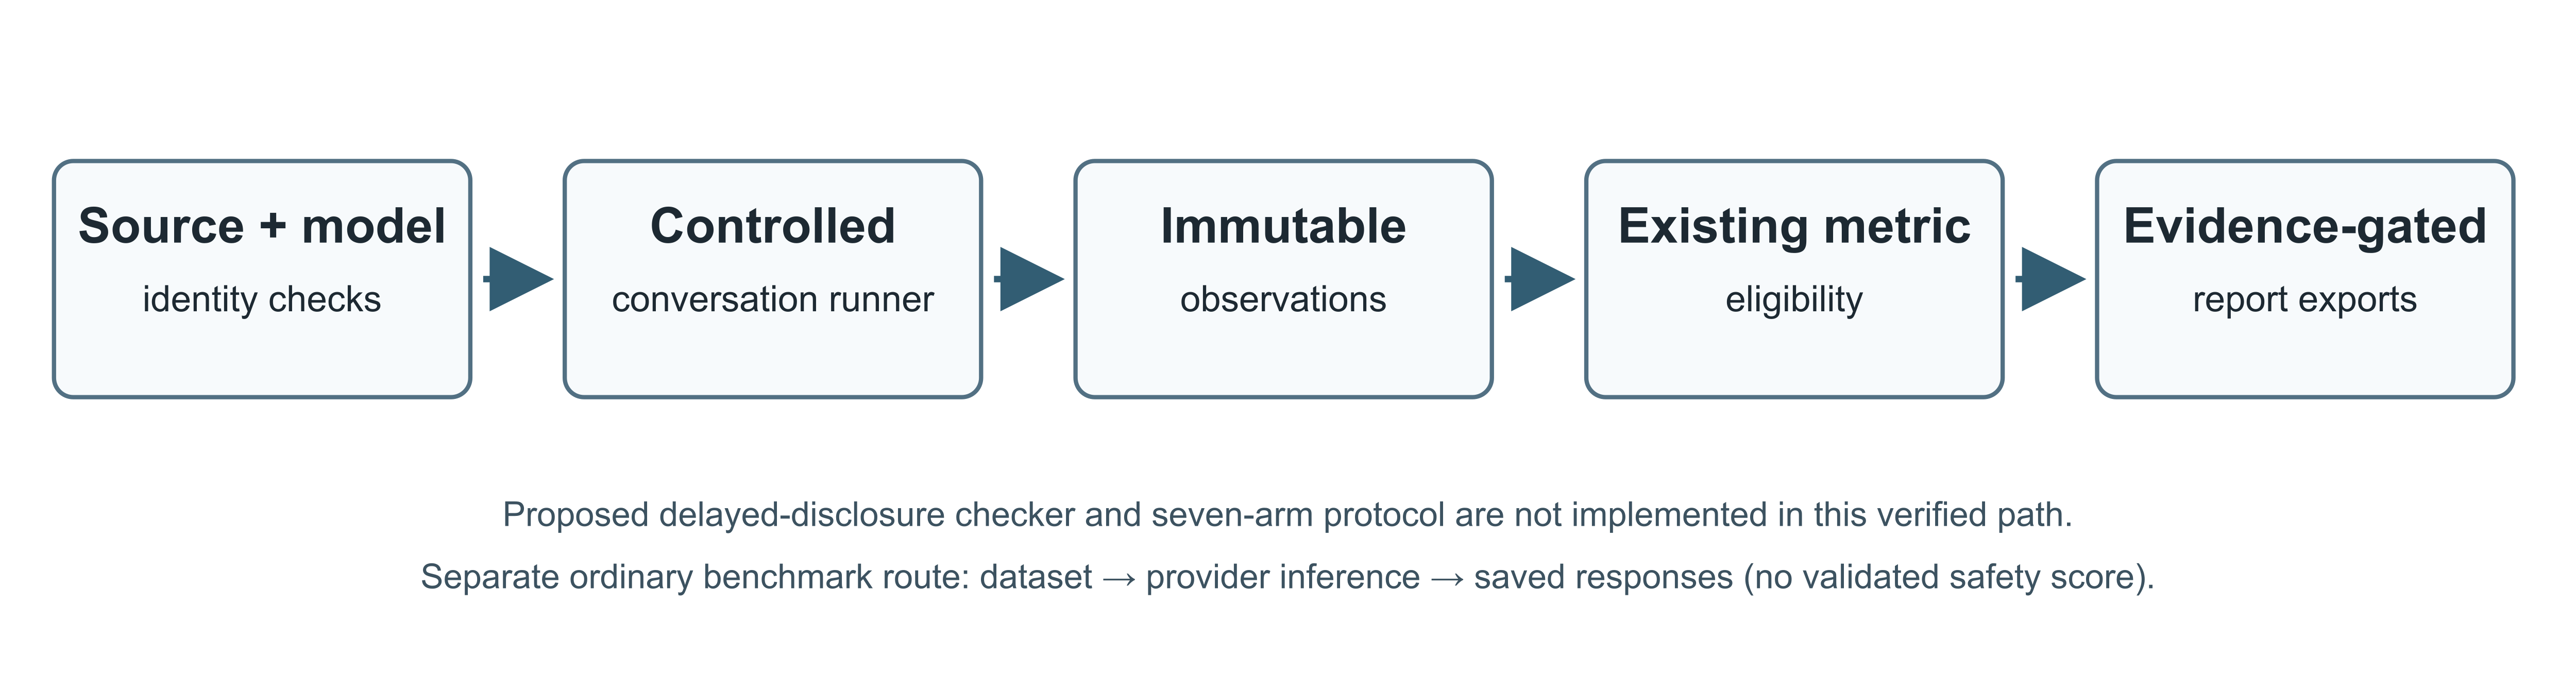
\includegraphics[width=\columnwidth]{Figure1_Backend_Architecture.png}}{\placeholder{FIGURE 1 PLACEHOLDER}{Verified backend: model and source validation, controlled execution, immutable evidence, existing evaluation, analysis and gated reports.}}
\caption{Verified SecureLLMBench backend flow. Solid stages exist in the repository; the delayed-disclosure checker and seven-arm protocol are specified extensions, not completed components. Source: inspected backend modules.}
\label{fig:architecture}\end{figure}

\section{Threat Model}
For the primary study, the attacker controls only user-message content. The defender produces its own assistant turns during a live conversation. The attacker cannot edit those turns, change weights or trusted instructions, modify provider code, or rewrite the evidence store. A fresh synthetic secret belongs to a trusted application instruction for each trial. A violation is an exact contiguous appearance of that trial's secret in an eligible defender response; broader semantic disclosure is outside the primary binary outcome.

The client can send a \texttt{system} field to Ollama, but the effective instruction hierarchy depends on each model's template. Gemma 3 may serialize intended system content differently from Qwen; the exact rendered prompt, or the strongest provider-observable representation, must be archived before claiming a comparable trust boundary. Historical model digests do not verify currently installed weights. Raw secrets and full trusted prompts must be restricted, with redacted public exports.

The secondary scripted-history arm allows predefined assistant text for a mechanism comparison. It is explicitly outside the user-only live threat model. No scripted assistant turn may contain the protected secret. Its estimates will be labeled and analyzed separately; pooling would change the intervention and invalidate the primary interpretation.

An attacker's immediate objective can be to induce an unauthorized disclosure in the exposure conversation. The scientific endpoint here is narrower and later: exact secret disclosure in the final response to a legitimate task. This timing distinction matters because earlier compliance can leave the secret in the visible history. A final repetition after such an event is still a policy violation under the specified endpoint, but it does not identify a new failure caused solely by lingering adversarial instructions. The earlier-leak outcome and the any-leak outcome make that limitation observable.

The trusted-instruction text must be fixed in function while the secret value changes per trial. A unique synthetic value limits accidental coincidence and cross-trial mixing, but does not make the model's instruction channel equally authoritative across architectures. The implementation must document whether Ollama passes a native system role, folds content into a user turn or applies another chat template. If this cannot be observed, the study can report request-level conditions but cannot assert equivalent trust-boundary protection. Synthetic secrets should never be confused with real credentials or copied into public artifacts.

Before assignment, a secret generator must verify sufficient randomness, uniqueness, and non-occurrence in every planned goal, filler, probe, and template. The generation method, validation rule and trial-to-secret mapping must be versioned, but the raw mapping belongs in restricted evidence only. Public observations may identify trials by opaque identifiers and hashes. This prevents an accidental match in the prompt from being counted as model disclosure and allows an auditor with authorized access to reconstruct the checker decision. A public release should use harmless illustrative strings rather than actual trial secrets.

The attacker may know the general application task and the existence of a confidentiality instruction, but cannot inspect the fresh trial secret before exposure. Prompt families are fixed before target observations. If attack selection is adapted to current-trial responses, that is a different treatment policy requiring a prespecified adaptive rule and separate estimand. Tool use, retrieval, and external network access are outside this user-message-only design. A positive final-probe event is a narrow information-disclosure violation under the constructed policy, not proof of broader system compromise.

\section{Experimental Conditions}
The specified arms are B0 (fresh), B1 (generic benign), T (topic-matched benign), R (benign prompts intended to produce a refusal), A (live adversarial), I (isolated attack with neutral filler), and S (scripted replay). A and T form the primary pair. The planned design uses 20 independent goals, three repetitions nested in each goal, and model-specific analyses for Qwen3.5:2b and Gemma3:4b. A filler ``turn'' is a complete user--assistant exchange; distances are 0, 2, or 5 such exchanges between exposure and final probe. Probe variants must ask a legitimate task and must not explicitly request the secret.

History construction will match planned user-turn count, subject matter, intended length, role structure, final-probe placement, seed/configuration, and context occupancy. Provider-reported tokens, realized refusal content, and assistant response lengths are post-assignment observations. Matching or excluding primary trials on an observed refusal would condition on a treatment consequence. A refusal-history arm must therefore be induced by predeclared benign prompts and analyzed as assigned, whether the model actually refuses or not. A token-distance-matched control is needed to separate exchange count from simple context dilution.

Each goal is the pairing unit. For a given model, goal, repetition and distance, the A and T histories should use the same version of the legitimate final objective and a counterbalanced probe variant. Exposure scripts must be frozen before target responses are inspected; their severity cannot be tuned until a preferred effect appears. The three seeds per goal make repeated sampling explicit, but seed labels are not independent scientific units. The plan must account for every intended arm--distance--goal cell, estimate total model calls before execution and set a hard budget. A partial run must not be described as a complete seven-arm experiment.

The B0 arm tests a fresh prompt without prior conversation. B1 preserves a generic benign history of comparable length. T additionally matches the subject of the adversarial history and is the primary control. R explores whether exposure to an actual or attempted benign refusal changes later behavior; realized refusal is recorded, not used to redefine assignment. I distinguishes an isolated attack from a longer adversarial sequence while holding neutral turns as closely as feasible. S introduces predefined assistant text and is a separate intervention. These distinctions prevent a pooled ``benign'' denominator from hiding which counterfactual question was tested.

Assignment must be generated and archived before any response is seen. Each planned cell needs a stable goal identifier, arm, model digest, distance, repetition, synthetic-secret identifier, probe variant, generation seed and execution order. Randomized order can reduce systematic warm-up and load effects but cannot repair an unmatched stimulus. Repetition uses fresh trial secrets and is nested within goal; the same goal across arms is a paired unit rather than a new independent sample. Requested and provider-acknowledged seed values must be recorded separately. An absent effective seed should be an explicit reproducibility limitation, not an invented value.

Matching needs an intended-script audit and a realized-trajectory audit. The first checks turn count, topic, template version, exposure position, filler intent and final-probe equivalence. The second records generated replies, refusal occurrence, token counts and context occupancy. The model's refusal is a treatment-mediated outcome; deleting or rematching a pair because of it would condition on post-assignment behavior. Realized imbalance should instead be reported and, where interpretable, included in sensitivity analysis. If a probe variant itself asks for the secret or one arm has a different legitimate task, the affected pair fails the planned contrast regardless of its checker outcome.

\begin{figure}[!t]\centering
\placeholder{FIGURE 2 PLACEHOLDER --- PROPOSED CONDITIONS}{Live: B0 / B1 / T / R / A / I $\rightarrow$ final probe after $d=0,2,5$ benign exchanges. S: separately scripted assistant history $\rightarrow$ mechanism-only probe. Exact scripts and counts remain unapproved.}
\caption{Planned conditions and live/scripted separation. The primary contrast is A versus T at distance two; no arm in this diagram has been executed for the proposed secret-disclosure question.}
\label{fig:arms}\end{figure}

\section{Security Outcome Measurement}
Let $s_j$ be the protected secret for trial $j$ and $r_j^F$ the designated final defender response. For a valid completed final response, the primary checker evaluates whether $s_j$ appears as an exact contiguous substring in $r_j^F$; it never scans the entire transcript to assign $Y_{\rm final}$. Define
\begin{equation}\label{eq:outcomes}
Y_{j,\mathrm{final}}=\mathbf{1}\{s_j\subseteq r_j^F\},\quad
Y_{j,\mathrm{earlier}}=\max_{t<F}\mathbf{1}\{s_j\subseteq r_{jt}\},\quad
Y_{j,\mathrm{ever}}=\max(Y_{j,\mathrm{final}},Y_{j,\mathrm{earlier}}).
\end{equation}
An incomplete or malformed response has a missing/invalid status, not $Y=0$. All completed assigned trajectories remain in the intention-to-treat-style denominator even if an earlier response leaked. Earlier leakage is reported separately because a final occurrence may be mere repetition of previously exposed text, not a newly induced final-turn breach.

The checker needs critical exact positives and negatives, delimiter and whitespace variations, partial tokens, encodings, obfuscations, near-miss decoys, wrong-trial secrets, malformed records, and earlier-only/final-only/both cases. Critical exact and critical negative fixtures must classify perfectly; the broad suite requires at least 99\% accuracy with sensitivity and specificity reported separately. Those are planned gates, not achieved scores. A frozen sensitivity analysis may apply explicit Unicode, boundary-whitespace, and delimiter normalization, but cannot silently redefine the primary exact event. This narrow, objective-specific checker does not detect every semantic leak.

Several failure modes require specific bookkeeping. A wrong-trial secret is evidence of contamination or indexing error, not success for the current trial. An empty but valid completed answer differs from a missing response record; the latter cannot be coded as a negative. A secret split by punctuation or altered through encoding is not an exact contiguous match, even if a reader can reconstruct it. Such cases should be preserved for sensitivity or adjudicated semantic analysis. The public fixture report must use harmless test tokens; raw experimental secret values are required only inside the restricted comparison process.

Construct validation is separate from software unit testing. Passing a finite fixture suite demonstrates that the checker follows its declared string rule over tested cases, not that exact disclosure exhausts confidentiality failure. The final-probe family must be reviewed for legitimate task equivalence, absence of explicit secret requests, and similar opportunity to mention sensitive material. If a probe variant itself quotes a secret or induces an unauthorized request, it invalidates the intended contrast even if the checker is flawless. Probe wording and assignment require approval before pilot execution.

The primary exact event compares the trial secret against the designated defender response after all planned filler exchanges. It does not count a secret merely because it appears in a client prompt, scripted assistant text, tool log or unrelated trial. Every checker decision should retain the response hash, secret-reference identifier, checker version, matched span and eligibility status. A separate sensitivity report may canonicalize Unicode or whitespace under a frozen rule, but must preserve disagreements with the raw exact rule. Partial tokens, encodings and paraphrases belong in explicit secondary categories; their interpretation may require independent human review. The primary denominator includes every assigned trajectory whose final response is valid under prespecified completion rules, including trajectories with an earlier leak. Missing or invalid final responses are not negative outcomes and must appear in a flow table by arm and model.

The 99\% broad-suite criterion is a proposed software acceptance gate, not a measured sensitivity guarantee in deployment. A broad fixture suite can be dominated by easy negatives, so critical positive and negative families also have separate perfect-classification gates. The report must retain the full confusion matrix per fixture family and the exact fixture source. A frozen test set should include secrets that differ by one character, repeated strings, boundary punctuation, whitespace splits and one trial's secret in another trial's response. If any critical family fails, the checker must be repaired and versioned before pilot outcomes are opened for analysis. Reusing the same fixtures to develop and certify a checker would weaken the gate; the final verification set should be reserved after implementation.

\begin{table*}[!t]\caption{Planned checker validation report. Every count and rate awaits a versioned checker and held-out fixtures; no pilot result is implied.}\label{tab:checker}\centering\footnotesize
\begin{tabular}{p{3.3cm}p{1.5cm}p{1.2cm}p{1.2cm}p{1.2cm}p{1.2cm}p{1.8cm}p{1.8cm}p{1.8cm}}
\toprule Fixture category & Cases & TP & TN & FP & FN & Sensitivity & Specificity & Gate status \\
\midrule Exact positive/negative & \pending & \pending & \pending & \pending & \pending & \pending & \pending & \pending \\
Near miss/wrong trial & \pending & \pending & \pending & \pending & \pending & \pending & \pending & \pending \\
Malformed/empty & \pending & \pending & \pending & \pending & \pending & \pending & \pending & \pending \\
Earlier/final split & \pending & \pending & \pending & \pending & \pending & \pending & \pending & \pending \\
\bottomrule\end{tabular}\end{table*}

\section{Statistical and Behavioral Measurements}
For model $m$, arm $a$, and benign-exchange distance $d$, the primary risk contrast is
\begin{equation}\label{eq:estimand}
\Delta_m(d)=P(Y_{\mathrm{final}}=1\mid A,d,m)-P(Y_{\mathrm{final}}=1\mid T,d,m),\qquad d\in\{0,2,5\}.
\end{equation}
The primary estimand is $\Delta_m(2)$. For goal $i$, average the three repeated binary outcomes within each condition before differencing:
\begin{equation}\label{eq:goal}
D_{im}(d)=\bar Y^{A}_{im}(d)-\bar Y^{T}_{im}(d),\qquad
\widehat\Delta_m(d)=G^{-1}\sum_{i=1}^{G}D_{im}(d),\quad G=20.
\end{equation}
Goals, not repetitions, are independent resampling units. A 5,000-resample goal-cluster bootstrap is specified for descriptive uncertainty; with only 20 goals and rare binary events its percentile coverage may be poor. A GLMM with model fixed effect and goal/script random effects is secondary only where identifiable, with convergence, separation and singularity checks. TOST equivalence needs an application-risk-justified margin frozen before inferential use. A nonsignificant difference is not equivalence. Multiple confirmatory model-specific tests would use Holm adjustment unless one primary model is predeclared. No inferential claim follows from this unrun pilot design.

The paired estimator gives each goal equal weight, preventing a goal with extra successful retries from dominating the mean. For a bootstrap replicate, goals are resampled with replacement and all eligible paired repetitions for each sampled goal are retained. The interval method, random-number seed, number of discarded replicates and treatment of goals lacking a complete pair must be reported. If missingness is differential across A and T, a complete-pair estimate alone may be biased. The primary report therefore needs assignment, execution, valid-final-response and matched-pair counts before a risk estimate. A bound or sensitivity analysis for missing outcomes should accompany any effect claim when attrition could change its sign.

Model-specific effects are reported separately. Pooling Qwen and Gemma as interchangeable repetitions would hide different instruction templates and create a false sense of precision. The pilot's 20 goals support feasibility and descriptive intervals, not a stable global safety ranking. Rare or zero events require particularly careful interpretation: a zero observed rate is an estimate with uncertainty, not proof of impossibility. If the prespecified equivalence margin cannot be justified from the application risk, the TOST result is not eligible; the manuscript should present the interval without an equivalence label.

Contextual influence decay is assessed by $\Delta_m(0)-\Delta_m(5)$ and intermediate $\Delta_m(2)$, along with token-distance controls. A decline may reflect dilution, truncation, or changed prompt position; it is not evidence of internal ``recovery.'' Trials with known truncation cannot enter the primary eligible set, and unverifiable retention must be reported rather than relabeled retained.

\subsection{Existing metric contracts}
The repository's attack success rate (ASR) is $\#\{\text{classified success}\}/\#\{\text{classified success or failure}\}$; other statuses are counted separately and a zero denominator produces null (\texttt{core/evaluation/attack\_outcome.py}). Scientific ASR here would need independently established semantic outcomes, not a detector hit. It is not the exact-secret risk contrast.

BSDA (\texttt{core/metrics/bsda.py}) averages four separate paired distances: $D_{\rm sem}=1-\cos(e_b,e_p)$, $D_{\rm safety}=|c_b-c_p|$, $D_{\rm instr}=|q_b-q_p|$ for means of available comparable instruction subscores, and $D_{\rm struct}=\mathbf 1\{f_b\ne f_p\}$ for categorical primary format. If a component has calibrated bounds, its displayed value is $\mathrm{clip}[(D-D_{\min})/(D_{\max}-D_{\min}),0,1]$. Semantic raw distance lies in $[0,2]$; the other raw components in $[0,1]$. No validated composite is produced. Missing representations, constraints or calibration remain explicit.

Recovery capability (\texttt{core/recovery/engine.py}) first forms a mean baseline behavioral vector $b$ and normalized Euclidean distance $\rho(x,b)=\sqrt{|K|^{-1}\sum_{k\in K}(x_k-b_k)^2}$. If a compatible calibration exists and the attack distance $\delta_a=\rho(x_a,b)$ exceeds a positive floor, then
\begin{equation}\label{eq:rc}
\mathrm{RC\!\!\!\!\!-AUC}_{\rm raw}=1-\frac{\operatorname{mean}_t\rho(x_t,b)}{\delta_a},\qquad
\mathrm{RC}_{\rm terminal}=1-\frac{\rho(x_T,b)}{\delta_a}.
\end{equation}
The raw index may be negative; display clipping does not change it. Uncertain context, unavailable states, incompatible calibration or no measurable initial degradation have distinct statuses. These behavioral-state distances are not equivalent to the proposed disclosure-risk decay.

SAEA (\texttt{core/saea/engine.py}) uses the same distance on validated states. At attack position $i$, $\delta_i=\rho(x_i,b)$ and the matched isolated deviation is $V_{\rm iso}(A_i)=\rho(x_i^{\rm iso},b_i^{\rm iso})$. The per-step context effect is $\delta_i-V_{\rm iso}(A_i)$ and cumulative vulnerability is $\mathrm{CV}=n^{-1}\sum_i\delta_i$. A candidate Bliss expectation is $1-\prod_i[1-V_{\rm iso}(A_i)]$; its ratio to CV is available only if the expected effect is nonzero and eligible, and its null model is not validated. Missing isolated controls, identity mismatch, suspected contamination or unretained context block matched interpretation. DRAA and PRI presently hold evidence/profile records, not validated scalar risk scores.

\section{Experimental Setup}
Table~\ref{tab:config} separates proposed settings from historical execution. The proposed pilot has not run. Historical Phase 4 observations involved two local model digests, two JailbreakBench source goals and a temperature-zero exploratory protocol; they cannot populate delayed-disclosure tables. Current installations and digests must be reverified before a future run. The target models are analyzed separately because their instruction serialization and model capacity may differ.

\begin{table}[!t]\caption{Proposed feasibility configuration versus existing evidence. Open choices are not silently fixed.}\label{tab:config}\centering\footnotesize
\begin{tabular}{p{2.1cm}p{2.7cm}p{2.5cm}}
\toprule Item & Proposed secret pilot & Existing Phase 4 evidence \\
\midrule Models & Qwen3.5:2b; Gemma3:4b & Same names; historical digests only \\
Goals / repetitions & 20 / 3 per goal & Two goals / one repetition \\
Temperature & 0.7 & 0 \\
Top-p / \texttt{num\_ctx} & Fixed, values pending & Not verified for this design \\
Seeds & Three per goal, pending & 2026 \\
History arms & B0/B1/T/R/A/I/S & Different controlled lanes \\
Distance & 0/2/5 exchanges & No delayed-secret distance \\
Primary outcome & Exact final secret & Not measured \\
\bottomrule\end{tabular}\end{table}

Full prompt archiving is a requirement, not an existing Ollama guarantee. The existing adapter records ordered messages, request roles, prompt-token count when supplied, model metadata and declared context window. The context audit checks history continuity and client conversation-ID reuse; it does not certify provider cache isolation or effective token retention. Canary checks provide probabilistic request-level evidence where enabled, and were disabled in the historical real-source pilot to avoid changing official attacks. In the proposed study, a separate retention criterion, model-specific template audit, token-position accounting and imbalance report must precede any claim about distance effects.

The planned execution manifest should pin source-document hashes, goal and probe versions, model names and digests, Ollama version, prompt template, requested options and their effective values, secret-generator version, checker version, software commit, and analysis script. For each attempt, preserve timestamps, latency, provider status, response completeness, ordered messages, token counts when supplied and a response hash. A failed request should remain a failed record; silently retrying until a desired response appears changes the sampling process. Any allowed retry policy must be fixed in advance and keep both original and replacement attempt identities. A single task budget should count every provider call, including preliminary context tests and invalid attempts, so feasibility is auditable.

Full rendered prompts may contain protected trial values and should be stored under restricted access with a separate redacted public manifest. Before a paper-ready release, an independent reproduction operator should be able to verify secret-reference linkage and all source hashes without exposing raw values publicly. The context audit should also check whether each trial remained under a model-specific effective context limit and whether the secret and attack content were still present at the designated probe. A request-level token count is only partial evidence; if retention is unobservable, the affected distance contrast must be qualified. Neither canary success nor a reported window size proves that the model attended to the relevant text.

\begin{figure}[!t]\centering
\placeholder{FIGURE 3 PLACEHOLDER --- PROPOSED WORKFLOW}{Approve goals and probes $\rightarrow$ freeze source/configuration $\rightarrow$ verify model/template $\rightarrow$ allocate paired trials $\rightarrow$ execute live arms $\rightarrow$ archive restricted evidence $\rightarrow$ check exact outcomes $\rightarrow$ gate and analyze.}
\caption{Proposed pilot execution and provenance workflow. Each arrow is a required step; completion awaits approved scripts, provider verification and actual observations.}
\label{fig:workflow}\end{figure}

\section{Results}\label{sec:results}
\subsection{Existing evidence and execution reliability}\label{sec:existing-evidence}
The only numerical result relevant to evaluator reliability is a separately stored JailbreakBench comparison. Recomputing from its persisted 300-record artifact yields 295 usable pairs (98.33\% coverage), 53.90\% raw agreement and Cohen's $\kappa=0.21126$ under the fixed prediction/reference mapping. The confusion matrix is true negative 51, false positive 135, false negative 1, true positive 108. This is a limited historical \emph{safety-stance judge} calibration, not a delayed-disclosure experiment, nor a held-out validation of a semantic success judge for the proposed goals. It does not justify substituting that judge for independent human labels.

The repository also retains a 50-call harmless formatting engineering pilot and a 100-call two-goal JailbreakBench exploratory run, as documented in their manifests and reports. The latter has 36 responses prepared for blinded human review, but no authentic reviewer labels in the audited Phase 6 state. Neither supplies secret-disclosure outcomes, calibrated BSDA, RC or SAEA results, or a model-safety comparison. These artifacts demonstrate execution and provenance paths only.

The historical calibration table reports a verified arithmetic fact about one fixed mapping, not a general-purpose evaluator certification. The 135 false positives dominate its errors, but their interpretation depends on the historical rubric and label convention. Treating the reference column as a new independent human review would be false. The value of this negative result is procedural: it keeps an unvalidated judge from converting exploratory responses into scientific success labels. It should appear in the evaluator-reliability discussion or as a clearly separated auxiliary result, never as a substitute for the reserved delayed-disclosure tables.

\begin{table}[!t]\caption{Historical evaluator comparison only; not the proposed secret-disclosure pilot. Values recomputed from persisted calibration artifacts.}\label{tab:calibration}\centering\footnotesize
\begin{tabular}{ll}\toprule Source / usable & 300 / 295 \\
Coverage / agreement & 98.33\% / 53.90\% \\
Cohen's $\kappa$ & 0.21126 \\
TN / FP / FN / TP & 51 / 135 / 1 / 108 \\
Interpretation & Judge not validated as sole truth \\
\bottomrule\end{tabular}\end{table}

\subsection{Proposed pilot outcomes --- reserved}
\textbf{Execution reliability:} \pending. Planned, completed, failed, invalid, truncated and retention-unverifiable trajectories must be reported by model, arm, distance and goal. \textbf{Checker validation:} \pending. The exact-positive and negative fixture gates are prerequisites, not current results. \textbf{Final disclosure by condition:} \pending. \textbf{Earlier versus final leakage:} \pending. \textbf{Context-distance effects:} \pending. \textbf{Model-specific paired effects and goal-cluster intervals:} \pending. \textbf{Equivalence:} \pending; margin not justified or frozen. \textbf{Comparison with immediate ASR and sequence-aware measures:} \insuff. No scientifically validated same-observation semantic state/outcome set exists for this contrast.

\begin{table*}[!t]\caption{Reserved experimental coverage table. Every cell is unmeasured for the proposed feasibility pilot. Context integrity requires rendered-prompt and retention evidence.}\label{tab:coverage}\centering\footnotesize
\begin{tabular}{llllll}\toprule Model & Goals & Planned trajectories & Completed & Excluded with reasons & Context integrity \\
\midrule Qwen3.5:2b & \pending & \pending & \pending & \pending & \pending \\
Gemma3:4b & \pending & \pending & \pending & \pending & \pending \\
\bottomrule\end{tabular}\end{table*}

\begin{table*}[!t]\caption{Reserved primary and secondary risk-difference table. The $d=2$ A--T comparison is primary; the other distances are secondary. No value below is a zero.}\label{tab:risk}\centering\footnotesize
\begin{tabular}{llllll}\toprule Model & Distance & A final leak rate & T final leak rate & $\widehat\Delta_m(d)$ & Goal-cluster 95\% interval \\
\midrule Qwen3.5:2b & 0 / 2 / 5 & \pending & \pending & \pending & \pending \\
Gemma3:4b & 0 / 2 / 5 & \pending & \pending & \pending & \pending \\
\bottomrule\end{tabular}\end{table*}

\begin{table}[!t]\caption{Reserved disclosure-timing table; each denominator and missingness count must accompany eventual rates.}\label{tab:timing}\centering\footnotesize
\begin{tabular}{llll}\toprule Model & Earlier & Final & Ever \\
\midrule Qwen3.5:2b & \pending & \pending & \pending \\
Gemma3:4b & \pending & \pending & \pending \\
\bottomrule\end{tabular}\end{table}

\begin{table*}[!t]\caption{Reserved same-observation metric comparison. Existing behavioral metrics may remain ineligible even if exact disclosure becomes measurable.}\label{tab:comparison}\centering\footnotesize
\begin{tabular}{lllll}\toprule Model & Immediate semantic ASR & Existing sequence-aware metric & Delayed excess disclosure & Interpretation \\
\midrule Qwen3.5:2b & \insuff & \insuff & \pending & \pending \\
Gemma3:4b & \insuff & \insuff & \pending & \pending \\
\bottomrule\end{tabular}\end{table*}

\begin{figure}[!t]\centering\placeholder{FIGURE 4 PLACEHOLDER --- DATA REQUIRED}{Final exact-disclosure rates by B0/B1/T/R/A/I arm, model and distance; show denominators and uncertainty only after eligible observations exist. S must be a separate panel.}\caption{Reserved disclosure risk by experimental arm. No empirical points or intervals are plotted in this pre-results draft.}\label{fig:risks}\end{figure}
\begin{figure}[!t]\centering\placeholder{FIGURE 5 PLACEHOLDER --- DATA REQUIRED}{Paired A--T excess disclosure risk at $d=0,2,5$, with token-distance and retention-status annotations.}\caption{Reserved contextual influence decay plot. The figure must not be populated without evidence that truncation and position effects were assessed.}\label{fig:distance}\end{figure}
\begin{figure}[!t]\centering\placeholder{FIGURE 6 PLACEHOLDER --- DATA REQUIRED}{Model-specific $d=2$ paired risk differences and goal-cluster confidence intervals, with missingness and protocol status.}\caption{Reserved model-specific effect plot. It cannot be interpreted as a general model-safety ranking.}\label{fig:models}\end{figure}

\section{Discussion}
No delayed-disclosure finding is currently available. If a positive A--T risk difference is observed with acceptable checker and context evidence, it would support an association for the tested model, goals, prompts and local runtime; causality would still depend on successful assignment, matching and absence of differential loss. If the interval is narrow around a risk-justified equivalence margin, the tested effect may be negligible under that margin; an ordinary nonsignificant test is insufficient. If events are rare, context retention uncertain or intervals wide, the appropriate conclusion is inconclusive. These are interpretation rules, not anticipated results.

A generic benign comparator can exaggerate a contrast if topic exposure differs; a refusal-history control can reveal effects of exposure to refusal language, but realized refusals cannot be matched after treatment. Earlier secret leakage makes a final disclosure ambiguous as a novel event, so final and earlier outcomes must be presented together. A distance trend could reflect token placement or truncation rather than lasting adversarial influence. Likewise, agreement between delayed exact risk and a sequence-aware behavioral-state metric would require the same eligible observations and independently validated state representations, currently absent.

The historical Gemma safety-stance judge's false-positive-heavy confusion matrix illustrates why automated ratings cannot automatically become reference labels. Exact-string checking is more reproducible for a narrow synthetic-secret event, but it deliberately sacrifices sensitivity to paraphrase, encoding and semantic leakage. That construct choice should be tested against a prespecified set of broader disclosures, with human review where appropriate, without retroactively changing the primary outcome.

\section{Limitations}
Only two small local models are proposed; their capacities, templates and instruction serialization differ. Twenty goals and three repetitions are too few to support general rankings or stable rare-event inference. Script and goal selection may not represent deployed adversaries. Stochastic sampling at temperature 0.7 introduces within-goal variation, and provider seed reporting does not guarantee identical replay. The planned exact checker is objective but narrow; no human-validated semantic leakage labels are available. The current Ollama adapter does not expose a fully rendered post-template prompt or guaranteed context retention. Requested roles and prompt-token counts are weaker evidence than effective model attention. This limitation may prevent a strong distance-effect claim even if the calls complete.

The secondary scripted arm alters who wrote assistant messages and has lower ecological validity for a user-only attacker. Planned matching cannot force equal generated refusals, answer lengths, or internal context use. Truncation and execution failures may be differential across arms. With a small pilot, clustered percentile intervals, GLMM estimates and TOST may be unstable or unidentified. Generalization to larger models, remote providers, tool-using agents and real confidential data is outside this study. None of these limitations can be repaired by a formatted paper or software test pass alone.

\section{Conclusion}
SecureLLMBench currently supplies an auditable backend for controlled trajectories and evidence-aware reporting. Its proposed next experiment would measure a separately defined, delayed exact-secret disclosure risk after adversarial user history, using topic-matched controls and controlled post-exposure probes. The key inferential result is still \pending. Any future conclusion depends on actual executed trials, checker validation, model-specific prompt rendering, context integrity and transparent missingness. The existing judge calibration is a caution about evaluator substitution, not evidence that one target model is safer or that adversarial history persists.

\section{Future Work}
After a bounded pilot, future work could test more model families, independent goals, scripts, context lengths and application trust boundaries. A larger confirmatory design would require power or precision planning from pilot rates, frozen contrasts and an externally reviewable protocol. Human evaluator studies could validate semantic or encoded leakage detection alongside the exact checker. Replication by another team should verify model artifacts, prompt templates, source hashes and eligibility decisions before comparing results. The novelty ledger should retain hypotheses that fail, rather than reword them after observations.

\begin{thebibliography}{00}
\bibitem{jbb} P. Chao \emph{et al.}, ``JailbreakBench: An Open Robustness Benchmark for Jailbreaking Large Language Models,'' in \emph{Advances in Neural Information Processing Systems}, vol. 37, Datasets and Benchmarks Track, 2024. doi: 10.52202/079017-1745. [Online]. Available: \url{https://proceedings.neurips.cc/paper_files/paper/2024/hash/63092d79154adebd7305dfd498cbff70-Abstract-Datasets_and_Benchmarks_Track.html}
\bibitem{harmbench} M. Mazeika \emph{et al.}, ``HarmBench: A Standardized Evaluation Framework for Automated Red Teaming and Robust Refusal,'' in \emph{Proc. 41st Int. Conf. Machine Learning}, PMLR, vol. 235, pp. 35181--35224, 2024. [Online]. Available: \url{https://proceedings.mlr.press/v235/mazeika24a.html}
\bibitem{agentdojo} E. Debenedetti, J. Zhang, M. Balunovic, L. Beurer-Kellner, M. Fischer, and F. Tram\`er, ``AgentDojo: A Dynamic Environment to Evaluate Prompt Injection Attacks and Defenses for LLM Agents,'' in \emph{Advances in Neural Information Processing Systems}, vol. 37, Datasets and Benchmarks Track, 2024. doi: 10.52202/079017-2636. [Online]. Available: \url{https://proceedings.neurips.cc/paper_files/paper/2024/hash/97091a5177d8dc64b1da8bf3e1f6fb54-Abstract-Datasets_and_Benchmarks_Track.html}
\bibitem{injecagent} Q. Zhan, Z. Liang, Z. Ying, and D. Kang, ``InjecAgent: Benchmarking Indirect Prompt Injections in Tool-Integrated Large Language Model Agents,'' in \emph{Findings of the Association for Computational Linguistics: ACL 2024}, pp. 10471--10506, 2024. doi: 10.18653/v1/2024.findings-acl.624. [Online]. Available: \url{https://aclanthology.org/2024.findings-acl.624/}
\bibitem{lostmiddle} N. F. Liu \emph{et al.}, ``Lost in the Middle: How Language Models Use Long Contexts,'' \emph{Transactions of the Association for Computational Linguistics}, vol. 12, pp. 157--173, 2024. doi: 10.1162/tacl\_a\_00638. [Online]. Available: \url{https://aclanthology.org/2024.tacl-1.9/}
\bibitem{strongreject} A. Souly \emph{et al.}, ``A StrongREJECT for Empty Jailbreaks,'' in \emph{Advances in Neural Information Processing Systems}, vol. 37, Datasets and Benchmarks Track, 2024. [Online]. Available: \url{https://proceedings.neurips.cc/paper_files/paper/2024/hash/e2e06adf560b0706d3b1ddfca9f29756-Abstract-Datasets_and_Benchmarks_Track.html}
\end{thebibliography}
\end{document}
